\begin{pastexam}[label={px:gk3-101-ds-03}]{高考三級資訊處理 101 年 第三題}
（申論；25 分）

堆積（heap）是一棵完整二元樹（complete binary tree），每個節點儲存一個鍵值（key value），且每一個
內部節點（internal node）的鍵值都不比其子節點的鍵值小。
\begin{itemize}[leftmargin=2em, labelsep=0.3em, itemsep=2pt]
\item[㈠] 請畫一棵七個節點的堆積，其節點儲存的鍵值形成的集合為 $\{100, 10, 55, 69, 38, 27, 48\}$。
（5 分）
\item[㈡] 請說明如何利用陣列（array）實做一棵 $n$ 個節點的堆積。（5 分）
\item[㈢] 假設一棵 $n$ 個節點的完整二元樹，其每個節點儲存一個鍵值，除了根節點（root）之外，其他
內部節點的鍵值均不比其子節點的鍵值小。請用虛擬碼描述將這樣的一棵二元樹調整成堆積的演算法。
（10 分）
\item[㈣] 請說明如何利用上述演算法將一棵 $n$ 個節點之堆積的根節點儲存的鍵值刪除，得到一棵儲存其餘
$n-1$ 個鍵值的堆積。（5 分）
\end{itemize}
\end{pastexam}

\begin{pastsoln}
題目定義的是\textbf{最大堆積}：父節點 $\ge$ 子節點，根是最大值（資結書第~8.1~節）。

\textbf{㈠} 七個節點的完整二元樹剛好是三層滿的。 根必須是最大的 $100$；第二層放 $69$、$55$，
第三層各放兩個比它小的數。 一種答法：
\begin{center}
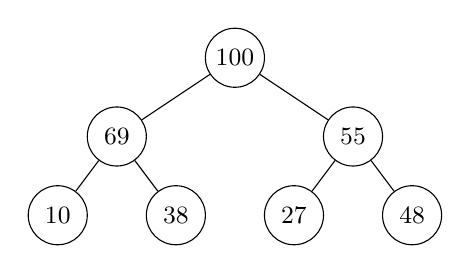
\begin{tikzpicture}[level distance=10mm,
  level 1/.style={sibling distance=30mm}, level 2/.style={sibling distance=15mm},
  every node/.style={circle, draw, minimum size=7.5mm, inner sep=0pt, font=\small}]
\node {100}
  child {node {69} child {node {10}} child {node {38}}}
  child {node {55} child {node {27}} child {node {48}}};
\end{tikzpicture}
\end{center}
檢查：$100 \ge 69, 55$；$69 \ge 10, 38$；$55 \ge 27, 48$，每個內部節點都不比子節點小。 答案不唯一，
例如 $69$ 和 $55$ 左右對調、或 $38$ 和 $48$ 對調也都是堆積；但根一定是 $100$，而且 $69$ 一定在
第二層（它只比 $100$ 小，放第三層的話它的父節點必須比它大，只能是 $100$，矛盾）。

\textbf{㈡ 用陣列存。} 完整二元樹由上到下、每層由左到右編號 $1, 2, \ldots, n$，節點 $i$ 存在
$A[i]$：
\begin{itemize}[nosep]
\item 節點 $i$ 的左子是 $2i$、右子是 $2i + 1$（$\le n$ 時才存在），父節點是 $\lfloor i/2 \rfloor$，
根是 $A[1]$。
\item 因為是完整二元樹，$A[1..n]$ 中間沒有空格，不必存指標；另外記一個變數 $n$ 表示目前的節點數。
\item 堆積性質寫成 $A[\lfloor i/2 \rfloor] \ge A[i]$，$2 \le i \le n$。
\end{itemize}
㈠ 的堆積存成 $A[1..7] = \langle 100, 69, 55, 10, 38, 27, 48 \rangle$。 （用 C 的 $0$ 起算陣列時，
子節點是 $2i+1$、$2i+2$，父節點是 $\lfloor (i-1)/2 \rfloor$。）

\textbf{㈢ 從根往下調整（sift-down，Heapify）。} 只有根可能比子節點小，其他地方都已經滿足堆積
性質，也就是根的左、右子樹各自都是堆積。 作法：把根和它較大的子節點比，若子節點比較大就交換，
問題就移到那個子節點；重複到不必交換或走到葉節點為止。
\begin{pseudo}{從節點 $i$ 往下調整成最大堆積}
\Procedure{Heapify}{$A, i, n$} \Comment{呼叫時用 $i = 1$}
    \While{$2i \le n$} \Comment{$i$ 還有子節點}
        \State $c \gets 2i$ \Comment{左子}
        \If{$c + 1 \le n$ \AND $A[c + 1] > A[c]$}
            \State $c \gets c + 1$ \Comment{右子比較大}
        \EndIf
        \If{$A[i] \ge A[c]$}
            \State \Return \Comment{已經不比子節點小，完成}
        \EndIf
        \State 交換 $A[i]$ 和 $A[c]$
        \State $i \gets c$ \Comment{往下繼續}
    \EndWhile
\EndProcedure
\end{pseudo}
\textbf{正確性}：迴圈不變量是「除了節點 $i$ 和它的子節點之間，整棵樹都滿足堆積性質」，而且
$i$ 的父節點（若有）$\ge$ $i$ 的子節點。 交換時把較大的子節點 $A[c]$ 拉上來，它 $\ge$ 另一個子
節點，也 $\ge$ 原來的 $A[i]$，所以 $i$ 這個位置滿足了；被換下去的值可能比 $c$ 的子節點小，問題
移到 $c$，不變量仍成立。 迴圈停在「$A[i] \ge$ 兩個子節點」或「$i$ 是葉節點」，這時整棵樹都滿足。
\textbf{時間}：每輪往下一層，最多走樹高 $\lfloor \lg n \rfloor$ 層，每層兩次比較，$O(\lg n)$
（資結書虛擬碼~8.1）。

\textbf{㈣ 刪除根。}
\begin{enumerate}[nosep]
\item 記下 $A[1]$（要刪除的最大值）。
\item 把最後一個節點 $A[n]$ 搬到根：$A[1] \gets A[n]$，$n \gets n - 1$。 這樣仍是 $n-1$ 個節點的
完整二元樹，只有根可能比子節點小，左右子樹本來就是堆積，正好是㈢的情況。
\item 呼叫 \proc{Heapify}($A, 1, n - 1$)。
\end{enumerate}
時間 $O(\lg n)$。 以㈠的堆積為例：刪除 $100$，把 $48$ 搬到根，得 $\langle 48, 69, 55, 10, 38, 27
\rangle$；$48$ 的子節點 $69$、$55$ 中較大的是 $69$，交換得 $\langle 69, 48, 55, 10, 38, 27 \rangle$；
$48$ 的子節點 $10$、$38$ 都比它小，停止。 結果 $69$ 在根，是其餘 $6$ 個鍵的堆積。
\end{pastsoln}
